% IEEE standard conference template; to be used with:
%   spconf.sty  - LaTeX style file, and
%   IEEEbib.bst - IEEE bibliography style file.
% --------------------------------------------------------------------------

\documentclass[letterpaper]{article}
\usepackage{spconf,amsmath,amssymb,graphicx}
\usepackage[norelsize]{algorithm2e}

\SetKwProg{Fn}{Function}{}{}

% Example definitions.
% --------------------
% nice symbols for real and complex numbers
\newcommand{\R}[0]{\mathbb{R}}
\newcommand{\C}[0]{\mathbb{C}}

% bold paragraph titles
\newcommand{\mypar}[1]{{\bf #1.}}

% Title.
% ------
\title{Optimization of Ant Colony Edge Detection algorithm}
%
% Single address.
% ---------------
\name{Hui Zhou} 
\address{DMAVT\\ ETH Z\"urich\\Z\"urich, Switzerland}

% For example:
% ------------
%\address{School\\
%		 Department\\
%		 Address}
%
% Two addresses (uncomment and modify for two-address case).
% ----------------------------------------------------------
%\twoauthors
%  {A. Author-one, B. Author-two\sthanks{Thanks to XYZ agency for funding.}}
%		 {School A-B\\
%		 Department A-B\\
%		 Address A-B}
%  {C. Author-three, D. Author-four\sthanks{The fourth author performed the work
%		 while at ...}}
%		 {School C-D\\
%		 Department C-D\\
%		 Address C-D}
%

\begin{document}
%\ninept
%
\maketitle
%

%The hard page limit is 6 pages in this style. Do not reduce font size
%or use other tricks to squeeze. This pdf is formatted in the American letter format, so may look a bit strange when printed out.

\begin{abstract}
%Describe in concise words what you do, why you do it (not necessarily
%in this order), and the main result.  The abstract has to be
%self-contained and readable for a person in the general area. You
%should write the abstract last.
In this paper, an ant-colony edge detection algorithm is implemented using the blocking strategy and non-repeated random number generator. An image is taken as an array to decrease the memory access and cache load of this algorithm. This approach speeds up the algorithm and can be extended in a parallel way.
\end{abstract}

\section{Introduction}\label{sec:intro}

%Do not start the introduction with the abstract or a slightly modified
%version. It follows a possible structure of the introduction. 
%Note that the structure can be modified, but the
%content should be the same. Introduction and abstract should fill at most the first page, better less.
%
%\mypar{Motivation} The first task is to motivate what you do.  You can
%start general and zoom in one the specific problem you consider.  In
%the process you should have explained to the reader: what you are doing,
%why you are doing, why it is important (order is usually reversed).
%
%For example, if my result is the fastest DFT implementation ever, one
%could roughly go as follows. First explain why the DFT is important
%(used everywhere with a few examples) and why performance matters (large datasets,
%realtime). Then explain that fast implementations are very hard and
%expensive to get (memory hierarchy, vector, parallel). 
%
%Now you state what you do in this paper. In our example: 
%presenting a DFT implementation that is
%faster for some sizes than all the other ones.
%
%\mypar{Related work} Next, you have to give a brief overview of
%related work. For a paper like this, anywhere between 2 and 8
%references. Briefly explain what they do. In the end contrast to what
%you do to make now precisely clear what your contribution is.

Ant Colony Edge Detection (ACED) is a heuristic approach for edge detection in image processing. Originated from ant colony optimization, it uses the pheromone trails generated by artificial ants to label the edges. In general, the ants are randomly distributed in an image and then moved by iterations. The ant movement is according to the transition probability \cite{nezamabadi2006edge, tian2008ant, LIU2015147},
\begin{equation*}
p^n_{ij\rightarrow \Omega_{ij}} =
\begin{cases}
\frac{\left(\tau_{rs}^{n-1}\right)^\alpha\left(\eta_{rs}\right)^\beta}{\sum_{rs}\left(\tau_{rs}^{n-1}\right)^\alpha\left(\eta_{rs}\right)^\beta} &\quad \text{if $(r,s)\in\Omega_{ij}$} \\
0 & \quad \text{otherwise} \\
\end{cases} 
\end{equation*}    
where $\tau^n_{ij}$ is the pheromone of the $n$th construction step at $(i,j)$ pixel position of the image and $\eta_{ij}$ is the heuristic information at that location. $\Omega_{ij}$ is the neighborhood of pixel $(i,j)$. $\alpha$ and $\beta$ are input parameters with typical value $\approx 2.0$. From this transition rule, we can see that the pixel with high heuristic information and pheromone will be frequently visited by the ants. After the movements of all ants, the pheromone $\tau^n_{ij}$ will be updated by
\begin{equation*}
\tau^n_{ij}\leftarrow(1-\rho)\tau^n_{ij}+\lambda
\end{equation*}
where $\rho$ is the pheromone evaporation rate and $\lambda$ is the pheromone left by the ants which visited this site. A typical setting of $\lambda$ \cite{nezamabadi2006edge, LIU2015147} is
\begin{equation*}
\lambda =
\begin{cases}
\sum_{k}\eta_{ij} & \text{if $k$th ant visited $ij$ and $\eta_{ij}\geq t$} \\
0 & \quad \text{otherwise} \\
\end{cases} 
\end{equation*}
where $t$ is a user-defined value to avoid noise. Due to the evaporation, the pheromone on the sites with low ant visiting frequency will eventually vanish so as to highlight the edges. In addition, each ant has memory length, which is to avoid the ant visiting previous positions stored in its memory. Besides this non-overlapping ant movement constraint, the initial ant position can also be randomly distributed over the region containing high heuristic information (e.g. $\eta_{ij}\geq t$) in a non-overlapping way.

In literature, Liu et al. \cite{LIU2015147} concluded that ACED yields better results than traditional edge detectors like Canny and Sobel but slower running speed. Some parallel ant colony optimizations are implemented using MPI \cite{RANDALL20021421}, OpenMP \cite{delisle2001parallel} and GPU \cite{dawson2014accelerating}. We refer to \cite{PEDEMONTE20115181} for a review of parallel approaches. In this paper, we used the blocking strategy to implement the ACED proposed in \cite{LIU2015147}. The algorithm is run on a single core and can be extended in parallel.    

\section{Background}\label{sec:background}

%Give a short, self-contained summary of necessary
%background information. For example, assume you present an
%implementation of FFT algorithms. You could organize into DFT
%definition, FFTs considered, and cost analysis. The goal of the
%background section is to make the paper self-contained for an audience
%as large as possible. As in every section
%you start with a very brief overview of the section. Here it could be as follows: In this section 
%we formally define the discrete Fourier transform, introduce the algorithms we use
%and perform a cost analysis.
%
%\mypar{Discrete Fourier Transform}
%Precisely define the transform so I understand it even if I have never
%seen it before.
%
%\mypar{Fast Fourier Transforms}
%Explain the algorithm you use.
%
%\mypar{Cost Analysis}
%First define you cost measure (what you count) and then compute the
%cost. Ideally precisely, at least asymptotically. In the latter case you will need to instrument your code to count
%the operations so you can create a performance plot.
%
%Also state what is
%known about the complexity (asymptotic usually) 
%about your problem (including citations).
%
%Don't talk about "the complexity of the algorithm.'' It's incorrect,
%remember (Lecture 2)?
The definition of heuristic information, according to \cite{LIU2015147}, is
\begin{equation*}
\eta_{ij}=\frac{\max|I_{i-u,j-v}-I_{i+u,j+v}|}{I_{\max}} \quad u,v \in \{-2,-1,0,1,2\}
\end{equation*}
where $I_{\max}$ is the maximum intensity value of gray-scale image $I$ and $I_{ij}$ is the intensity value of node $(i,j)$ in image $I$. Note that the range of $(u,v)$ value should be adjusted to $\{-1,0,1\}$ for the node $(i,j)$ near or at the boundary of image. For instance, the heuristic information at the upper boundary of image (without $2$ corners at the ends) degenerates to the normalized central difference $\eta_{ij}=\frac{|I_{i,j-1}-I_{i,j+1}|}{I_{\max}}$. Besides, the heuristic information is set to $0$ at the corners of image. Similarly, $\Omega_{ij}$, the neighborhood of node $(i,j)$, is defined as a $1$-ring around the node $(i,j)$,
\begin{equation*}
\Omega_{ij}=\{(r,s)\mid\max\{|u|,|v|\}=1, u=r-i, v=s-j\}
\end{equation*}
which means each ant has $8$ degrees of freedom for motion. However, it will decrease to $5$ at the boundaries and $3$ at the corners.

Combined all the ingredients mentioned before, with the proposed input parameter setting listed in Tab.\ref{tab:parameters}, 
\begin{table}[h!]
	\centering
	\begin{tabular}{|c|c|} 
		\hline
		image area & $A=\mathrm{height}*\mathrm{width}$ \\
		image perimeter & $P=2*(\mathrm{height}+\mathrm{width})$ \\
		initial $\tau_{ij}$ & $\tau_0 = 1\mathrm{e}-4$ \\
		number of ants & $K=\lfloor\sqrt{A}\rfloor$ \\
		ant moving steps & $L=\lfloor3\sqrt{A}\rfloor$ \\
		memory length & $M = \lfloor\sqrt{P}\rfloor$ \\
		$\tau$ power factor & $\alpha=2$ \\
		$\eta$ power factor & $\beta=2$ \\
		evaporation rate & $\rho=0.02$ \\
		$\eta$ threshold & $t = 0.1$ \\
		construction iterations & $N = 3$\\ 
		\hline
	\end{tabular}
	\caption{Proposed parameter values for initialization, $\lfloor\cdot\rfloor$ is the floor function}
	\label{tab:parameters}
\end{table}
the implementation follows Alg.\ref{alg:ACED},
\begin{algorithm}
	\KwIn{Grayscale image of size $\mathrm{height}\times\mathrm{width}$ }
	\KwOut{Binary image of the edges}
	initialize the parameters, pheromone matrix $\tau_{ij}$ and heuristic information matrix $\eta_{ij}$\;
	\For(){k=0; k$<$K; k++}{
		$\mathrm{ants}_{k0}=\mathrm{Random}(k)$\;
	}
	\For(construction iterations){n=0;n<N;n++}{
		\For(get current position of ant){k=0; k$<$K; k++}{
			$q = \mathrm{ants}_{k0}$\;
			$i = q/\mathrm{width}$\;
			$j = q\%\mathrm{width}$\;
			\For(move L-1 steps){l=1; l$<$L; l++}{
				\For(calculate the transition probability){$rs\in\Omega_{ij}$}{
					$p^n_{ij\rightarrow \Omega_{ij}}$\; 
				}

				\If(avoid the position in memory){$ij_{\mathrm{old}}\in\Omega_{ij}$}{
					$p^n_{ij\rightarrow ij_{\mathrm{old}}}=0$\;
				}

				$p^n_{ij_{\max}}=\max\{p^n_{ij\rightarrow \Omega_{ij}}\}$\;

				\eIf(){$p^n_{ij_{\max}}==0$ $\mathrm{or}$ $\eta_{ij_{\max}}<t$}{
					$ij_{\mathrm{new}}=\mathrm{Random}(k)$\;
				}{
					$ij_{\mathrm{new}}=ij_{\max}$\;
				}
				$\mathrm{ants}_{kl}=i_{\mathrm{new}}*\mathrm{width}+j_{\mathrm{new}}$\;
			}
		}
		$\tau_{ij}\leftarrow(1-\rho)*\tau_{ij}+\sum_{kl}\eta_{\mathrm{ants}_{kl}}$\;
		$\mathrm{ants}_{k0}\leftarrow\mathrm{ants}_{k(l-1)}$\;
	}
	
	\caption{Ant Colony Edge Detection algorithm}\label{alg:ACED}
\end{algorithm}
where the $\mathrm{Random}$ function is implemented under the non-overlapping constraint as shown in Alg.\ref{alg:rand}.
\begin{algorithm}
	\Fn{$\mathrm{Random}$(k)}{	
		$c = 0$\;
		$q = 0$\;
		$r = \mathrm{rand}()\%A$\;
		\While{$q<k$ $\mathrm{and}$ $c<A$}{			
			$r = \mathrm{rand}()\%A$\;
			\For{q=0; q$<$k; q++}{
				\If{$\mathrm{ants}_{q0} == r$ $or$ $\eta_r < t$}{
					break\;                       
				}
			}
			$c$++\;
		}
	}
	\KwRet{$r$}\;
	\caption{Random function for the ant distribution}\label{alg:rand}
\end{algorithm}

To speed up the algorithm, the image $I$ is taken as a $1$-D array rather than a $2$-D matrix. In other words, the pixel position $(i,j)$ is zipped as $ij=i*\mathrm{width}+j$. This is beneficial for storing the positions of ants and generating the non-repeated random numbers. In detail, the $\mathrm{ants}_{kl}$ matrix stores the position of the $k$th ant at the $l$ th step in only $1$ float $ij$ rather than $2$ floats $(i,j)$. When the movement of ant need to be conducted, the float $ij$ can be unzipped to $2$ floats $(i,j)$ by integer division $i=ij/\mathrm{width}$ and integer mod $j=ij\%\mathrm{width}$. This will increase the floating point operations meanwhile decrease the memory access and the cache load. Moreover, the random number generated by $ij=\mathrm{rand}()\%A$ will have less chance of overlapping than $2$ separate random numbers generated by $i=\mathrm{rand}()\%\mathrm{height}$ and $j=\mathrm{rand}()\%\mathrm{width}$ because the period $A=\mathrm{height}*\mathrm{width}$ is larger than the periods $\mathrm{height}$ and $\mathrm{width}$.      

In addition, the binary image of the edges is obtained by using the threshold $\tau_{0}$. The sites with the higher pheromone $\tau_{ij}>\tau_0$ are labeled as the edges (black) otherwise the region (white).
\section{Blocking strategy}\label{sec:yourmethod}
To further speed up the algorithm, it is necessary to slice the large input image so that the matrices can be fit into the cache. Therefore, Alg.\ref{alg:ACED} is wrapped into a $\mathrm{Block}$ function with arguments $\eta$, $(x_0,y_0)$ and $(width, height)$. The block is defined by $[x_0,x_0+width]\times[y_0,y_0+height]$. Note that the heuristic information matrix $\eta_{ij}$ is initialized outside the $\mathrm{Block}$ function so that the heuristic information at the boundaries of sliced image is complete. It is better to check the value of $A$ and $\eta$ to make sure the block area $A>0$ and the block contains more than $1$ color type (i.e. $\#\{\eta_{ij}\mid\eta_{ij}>t, (i,j)\in[x_0,x_0+width]\times[y_0,y_0+height]\}>0$). Finally, the algorithm with blocking follows the structure in Alg.\ref{alg.block}, where the block size is $height\times width$ in comparison with the image size $\mathrm{Height}\times\mathrm{Width}$. 
\begin{algorithm}
	\KwIn{Grayscale image of size $\mathrm{Height}\times\mathrm{Width}$ }
	\KwOut{Binary image of the edges}
	assert($I_{\max}>0$)\;
	initialize heuristic information matrix $\eta_{ij}$\; 
	$b_x=width$\;
	$b_y=height$\;
	$x_1=\mathrm{Width}/width*width$\;
	$y_1=\mathrm{Height}/height*height$\;
	\For{$y_0=0$; $y_0<y_1$; $y_0+=b_y$}{
		\For{$x_0=0$; $x_0<x_1$; $x_0+=b_x$}{
			$\mathrm{Block}(x_0,y_0,b_x,b_y,\eta)$\;
		}
		\For{$x_0=x_1$; $x_0<\mathrm{Width}$; $x_0+=b_x$}{
			$\mathrm{Block}(x_0,y_0,\mathrm{Width}-x_1,b_y,\eta)$\;
		}
	}
	\For{$y_0=y_1$; $y_0<\mathrm{Height}$; $y_0+=b_y$}{
		\For{$x_0=0$; $x_0<x_1$; $x_0+=b_x$}{
			$\mathrm{Block}(x_0,y_0,b_x,\mathrm{Height}-y_1,\eta)$\;
		}
		\For{$x_0=x_1$; $x_0<\mathrm{Width}$; $x_0+=b_x$}{
			$\mathrm{Block}(x_0,y_0,\mathrm{Width}-x_1,\mathrm{Height}-y_1,\eta)$\;
		}
		
	}
	\caption{Blocking strategy for ACED}\label{alg.block}
\end{algorithm}    
%Now comes the ``beef'' of the paper, where you explain what you
%did. Again, organize it in paragraphs with titles. As in every section
%you start with a very brief overview of the section.
%
%For this class, explain all the optimizations you performed. This mean, you first very briefly
%explain the baseline implementation, then go through locality and other optimizations, and finally SSE (every project will be slightly different of course). Show or mention relevant analysis or assumptions. A few examples: 1) Profiling may lead you to optimize one part first; 2) bandwidth plus data transfer analysis may show that it is memory bound; 3) it may be too hard to implement the algorithm in full generality: make assumptions and state them (e.g., we assume $n$ is divisible by 4; or, we consider only one type of input image); 4) explain how certain data accesses have poor locality. Generally, any type of analysis adds value to your work.
%
%As important as the final results is to show that you took a structured, organized approach to the optimization and that you explain why you did what you did.
%
%Mention and cite any external resources including library or other code.
%
%Good visuals or even brief code snippets to illustrate what you did are good. Pasting large amounts of code to fill the space is not good.


\section{Experimental Results}\label{sec:exp}
The image testing is run on Intel i5-4690 CPU (3.50GHz, L1d cache: 32K, L1i cache: 32K, L2 cache: 256K, L3 cache: 6144K) with gcc 6.3.1 compiler (-O0 flag). The result of ACED algorithm is shown in Fig.\ref{fig:lena_ACED}}. ACED with or without blocking yields nearly the same run time when the image size is small (e.g. $1s$/$1s$ for $512\times512$ lena image) but significant run time difference when the image size is large (e.g. $5s/25s$ for $1024\times1024$ lena image). We can also see that the image color given by ACED is deeper than that given by its blocking. This is due to the fact that the ant movements are constrained inside each block rather than walking around the whole image. Therefore the overall pheromone distribution of ACED with blocking is more sparser than the original ACED. Despite of this, the blocked ACED still captures the features of image and has a faster speed than the original one.    
\begin{figure}\centering
		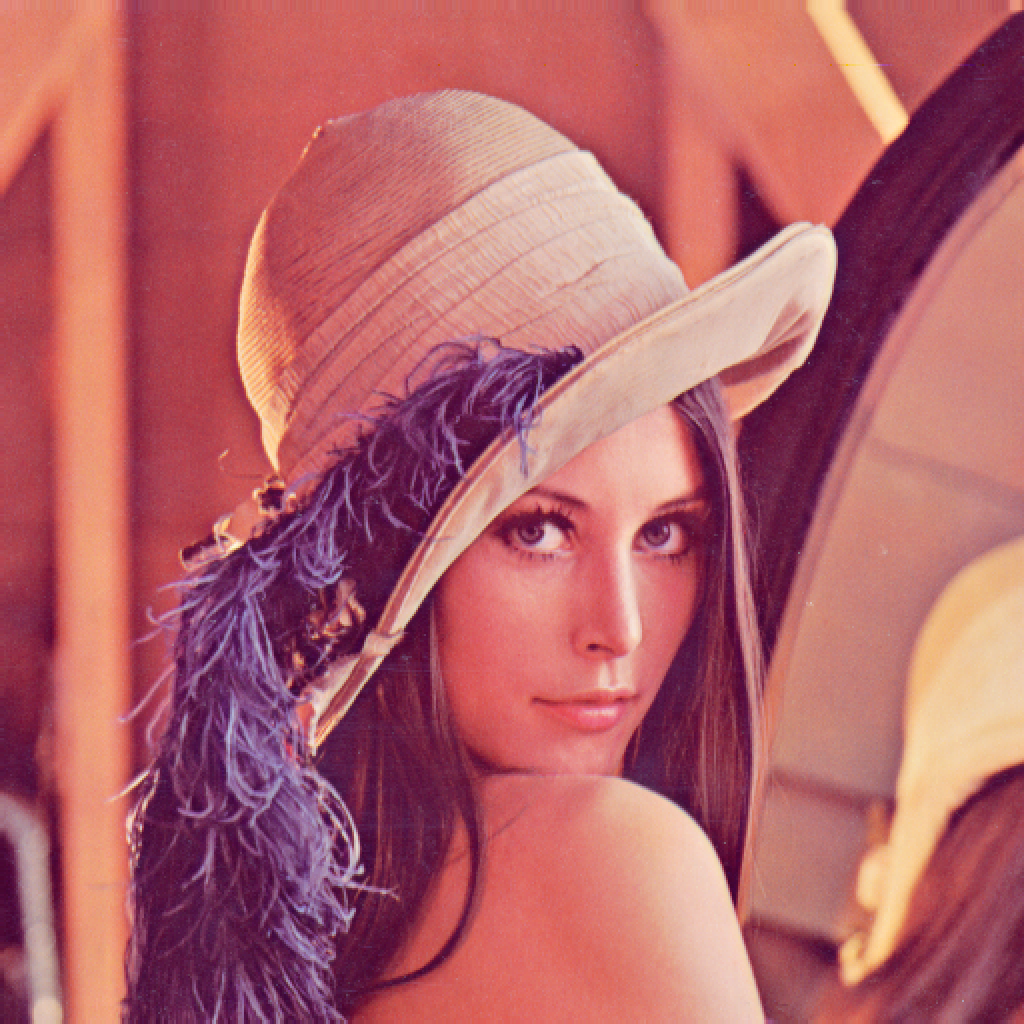
\includegraphics[width=0.3\columnwidth]{lena_std.png}
		%\caption{lena1024x1024 RGB image}\label{fig:lena}
		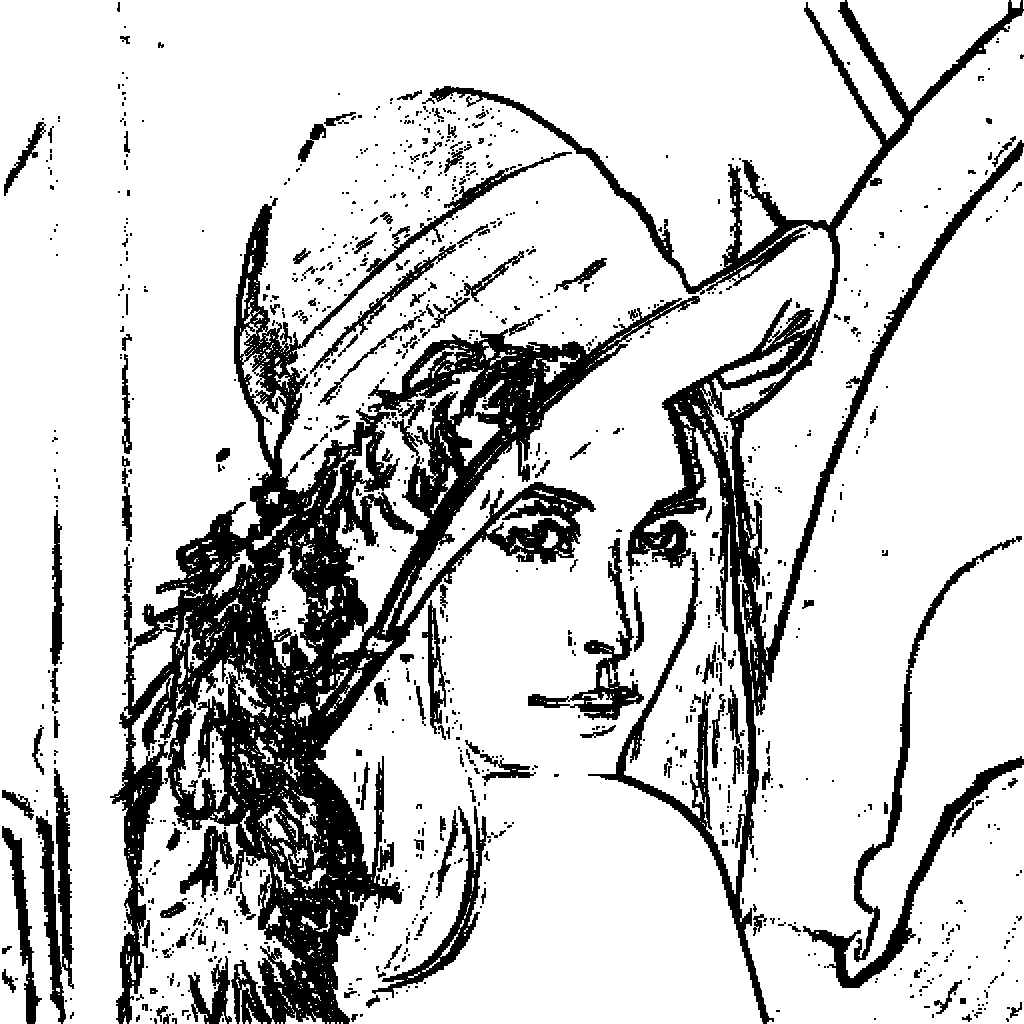
\includegraphics[width=0.3\columnwidth]{lena_std_test3.png}
		%\caption{ACED without blocking}\label{fig:lena_test}
		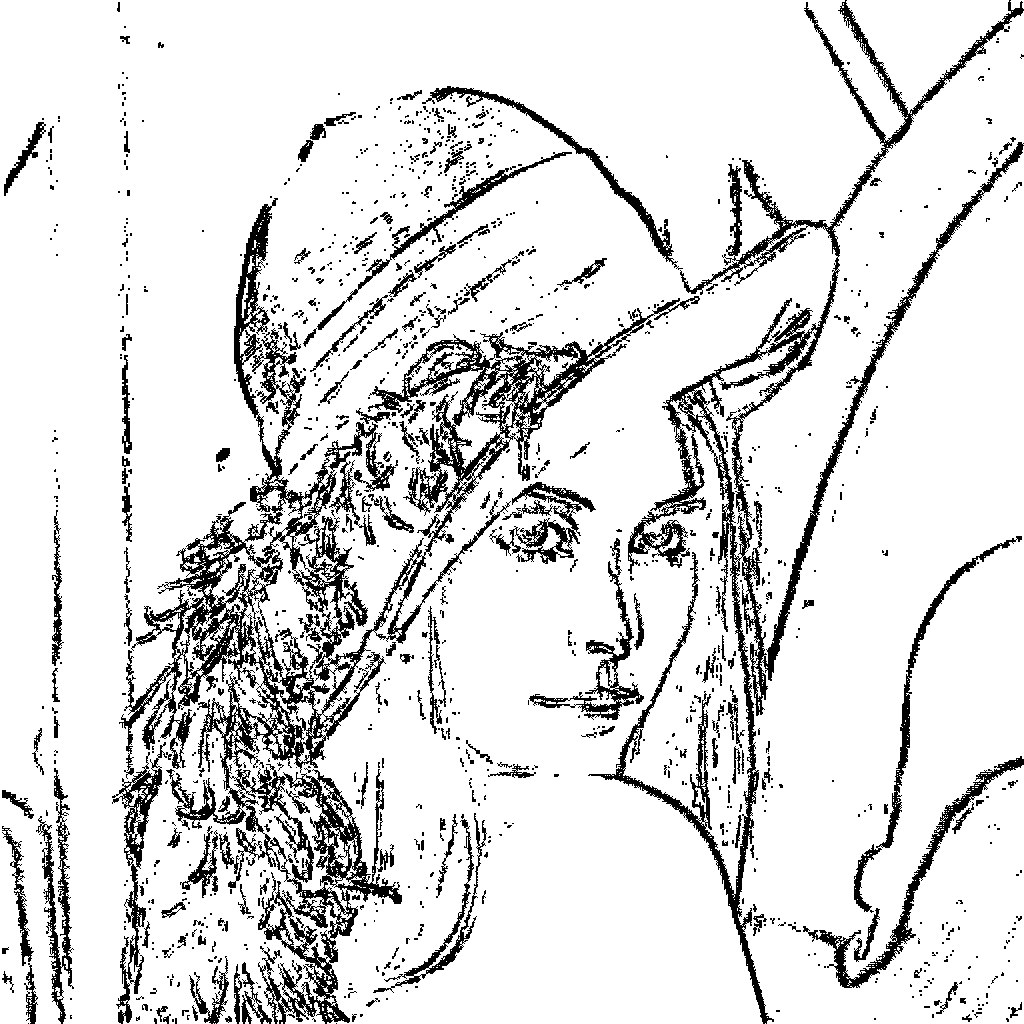
\includegraphics[width=0.3\columnwidth]{lena_std_testb1.png}
		%\caption{ACED with block size 256x256}\label{fig:lena_testb}
	\caption{lena image of size $1024\times1024$ (left); ACED (middle) and its blocking (right) run by Intel i5-4690 CPU with gcc 6.3.1 compiler -O0 flag}\label{fig:lena_ACED}
\end{figure} 

Furthermore, ACED with blocking is tested by an extreme case, that is, one black pixel image as shown in Fig.\ref{fig:Oneblackpixel_ACED}. We can hardly locate the black pixel by naked eyes, however, with the help of ACED, we can easily pinpoint its location. This has potential application in cosmology.     
\begin{figure}\centering
	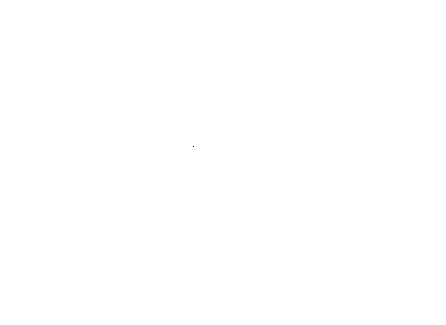
\includegraphics[width=0.3\columnwidth]{One_black_Pixel1.png}
	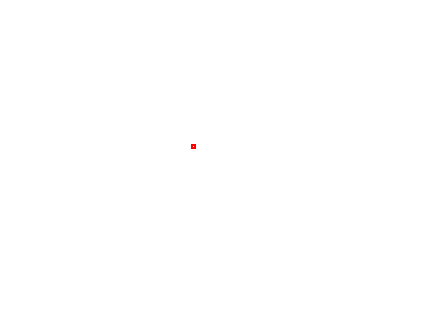
\includegraphics[width=0.3\columnwidth]{One_black_Pixel1_testb1.png}
	\caption{One black pixel image of size $325\times446$(left); blocked ACED circle out the black pixel in red color (right)}\label{fig:Oneblackpixel_ACED}
\end{figure} 
%Here you evaluate your work using experiments. You start again with a
%very short summary of the section. The typical structure follows.
%
%\mypar{Experimental setup} Specify the platform (processor, frequency, cache sizes)
%as well as the compiler, version, and flags used. I strongly recommend that you play with optimization flags and consider also icc for additional potential speedup.
%
%Then explain what input you used and what range of sizes. The idea is to give enough information so the experiments are reproducible by somebody else on his or her code.
%
%\mypar{Results}
%Next divide the experiments into classes, one paragraph for each. In the simplest case you have one plot that has the size on the x-axis and the performance on the y-axis. The plot will contain several lines, one for each relevant code version. Discuss the plot and extract the overall performance gain from baseline to best code. Also state the percentage of peak performance for the best code. Note that the peak may change depending on the situation. For example, if you only do additions it would be 12 Gflop/s
%on one core with 3 Ghz and SSE and single precision floating point.
%
%Do not put two performance lines into the same plot if the operations count changed significantly (that's apples and oranges). In that case first perform the optimizations that reduce op count and report the runtime gain in a plot. Then continue to optimize the best version and show performance plots.
%
%{\bf You should}
%\begin{itemize}
%\item Follow the guide to benchmarking presented in class, in particular
%\item very readable, attractive plots (do 1 column, not 2 column plots
%for this class), proper readable font size. An example is below (of course you can have a different style),
%\item every plot answers a question, which you pose and extract the
%answer from the plot in its discussion
%\end{itemize}
%Every plot should be discussed (what does it show, which statements do
%you extract).

\section{Conclusions}
The blocked ACED algorithm achieved comparable results and faster speed than the original one. It can be applied in cosmology to locate the stars from the image of galaxies. For the further optimization of this algorithm, some parallel approaches (e.g. MPI) can be used.  
%Here you need to briefly summarize what you did and why this is
%important. {\em Do not take the abstract} and put it in the past
%tense. Remember, now the reader has (hopefully) read the paper, so it
%is a very different situation from the abstract. Try to highlight
%important results and say the things you really want to get across
%(e.g., the results show that we are within 2x of the optimal performance ... 
%Even though we only considered the DFT, our optimization
%techniques should be also applicable ....) You can also formulate next
%steps if you want. Be brief.

%\section{Further comments}
%
%Here we provide some further tips.
%
%\mypar{Further general guidelines}
%
%\begin{itemize}
%\item For short papers, to save space, I use paragraph titles instead of
%subsections, as shown in the introduction.
%
%\item It is generally a good idea to break sections into such smaller
%units for readability and since it helps you to (visually) structure the story.
%
%\item The above section titles should be adapted to more precisely
%reflect what you do.
%
%\item Each section should be started with a very
%short summary of what the reader can expect in this section. Nothing
%more awkward as when the story starts and one does not know what the
%direction is or the goal.
%
%\item Make sure you define every acronym you use, no matter how
%convinced you are the reader knows it.
%
%\item Always spell-check before you submit (to me in this case).
%
%\item Be picky. When writing a paper you should always strive for very
%high quality. Many people may read it and the quality makes a big difference.
%In this class, the quality is part of the grade.
%
%\item Books helping you to write better: \cite{Higham:98} and \cite{Strunk:00}.
%
%\item Conversion to pdf (latex users only): 
%
%dvips -o conference.ps -t letter -Ppdf -G0 conference.dvi
%
%and then
%
%ps2pdf conference.ps
%\end{itemize}
%
%\mypar{Graphics} For plots that are not images {\em never} generate (even as intermediate step)
%jpeg, gif, bmp, tif. Use eps, which means encapsulate postscript, os pdf. This way it is
%scalable since it is a vector graphic description of your graph. E.g.,
%from Matlab, you can export to eps or pdf.
%
%Here is an example of how to get a plot into latex
%(Fig.~\ref{fftperf}). Note that the text should not be any smaller than shown.
%
%\begin{figure}\centering
%	\includegraphics[scale=0.33]{dft-performance.eps}
%	\caption{Performance of four single precision implementations of the
%		discrete Fourier transform. The operations count is roughly the
%		same. {\em The labels in this plot are too small.}\label{fftperf}}
%\end{figure}



% References should be produced using the bibtex program from suitable
% BiBTeX files (here: bibl_conf). The IEEEbib.bst bibliography
% style file from IEEE produces unsorted bibliography list.
% -------------------------------------------------------------------------
\bibliographystyle{IEEEbib}
\bibliography{bibl_conf}

\end{document}

